% Provenance (never printed): cycle 4 (geographie and SVT, "La planete Terre"):
% why a flat map distorts, projections, scale, topographic maps and
% profiles, satellite images and satellite positioning; see
% sources/book1/PROVENANCE.md. Book 1, grade 9, chapter 5.
% Vocabulary guard: owns map projection (Mercator, equal-area), numerical
% scale and scale bar, topographic map, contour line and contour interval,
% remote sensing and satellite image, satellite positioning. "Scale" itself
% is g2's (drawing-to-map, Sync 1 ruling); globe and world map are g3's;
% parallels, meridians, latitude and longitude are g6's; altitude, relief
% and physical map are g4's; slope as a percentage was used in g9.2. The
% speed of light is the physics books' (recalled in prose). The V-rule of
% geological maps belongs to Book 3.
\chapter{Mapas de toda la Tierra}\label{ch:g9:maps-of-the-earth}

En muchos \omterm{def:g2:drawing-to-map:map}{mapas} murales de clase, Groenlandia parece casi tan grande como
África. En un \omterm{def:g3:continents-and-oceans:globe}{globo terráqueo}, África es unas catorce veces mayor: unos
29~millones de kilómetros cuadrados para el \omterm{def:g3:continents-and-oceans:continent}{continente} africano, frente a
unos 2.1~millones para Groenlandia. Las dos son imágenes fieles de la
Tierra, hechas con cuidado. Entonces, ¿cuál de las dos miente, y por qué?
% ledger: data:ne-land (areas computed in figdata/grade-9/projections.py)

\begin{recall}
Un \omterm{def:g2:drawing-to-map:map}{mapa} es un dibujo de un lugar visto desde arriba, más pequeño que el
lugar, con una \omterm{def:g2:drawing-to-map:legend}{leyenda} y una \omterm{def:g2:drawing-to-map:scale}{escala} (\cref{ch:g2:drawing-to-map}). Un \omterm{def:g3:continents-and-oceans:globe}{globo
terráqueo} es una pequeña maqueta de la Tierra redonda; un \omterm{def:g3:continents-and-oceans:world-map}{mapamundi} muestra
toda la Tierra en plano, en una sola imagen
(\cref{ch:g3:continents-and-oceans}). Los \omterm{def:g6:latitude-longitude:latitude}{paralelos} y los \omterm{def:g6:latitude-longitude:longitude}{meridianos} dan a
cada lugar su \omterm{def:g6:latitude-longitude:latitude}{latitud} y su \omterm{def:g6:latitude-longitude:longitude}{longitud} (\cref{ch:g6:latitude-longitude}). La
\omterm{def:g4:world-physical-map:altitude}{altitud} es la altura sobre el \omterm{def:g4:world-physical-map:altitude}{nivel del mar}, y un \omterm{def:g4:world-physical-map:physical-map}{mapa físico} muestra el
\omterm{def:g4:world-physical-map:relief}{relieve} con colores (\cref{ch:g4:world-physical-map}). En física se aprende
que la luz viaja a unos \qty{300000}{km} por segundo.
\end{recall}
% ledger: const:c

\section{Por qué un mapa plano tiene que deformar}

Intenta aplanar la piel de una naranja sobre una mesa: se rompe o se
estira. La superficie de una esfera no puede extenderse en un plano sin
cambiar algunas longitudes. Para dibujar toda la Tierra en una hoja, el
cartógrafo elige una regla que envía cada punto del \omterm{def:g3:continents-and-oceans:globe}{globo} a un punto de la
hoja, y elige qué conservará fielmente el \omterm{def:g2:drawing-to-map:map}{mapa} y a qué renunciará.

\begin{definition}[Proyección cartográfica]\label{def:g9:maps-of-the-earth:projection}
Una \emph{proyección cartográfica}\index{proyeccion cartografica@proyección cartográfica}
es una regla que envía cada punto del \omterm{def:g3:continents-and-oceans:globe}{globo}, dado por su \omterm{def:g6:latitude-longitude:latitude}{latitud} y su
\omterm{def:g6:latitude-longitude:longitude}{longitud}, a un punto de un mapa plano. En una \emph{proyección de
Mercator}\index{proyeccion de Mercator@proyección de Mercator}, los
\omterm{def:g6:latitude-longitude:latitude}{paralelos} y los \omterm{def:g6:latitude-longitude:longitude}{meridianos} son rectas que se cortan en ángulo recto, y la
forma de cada región pequeña se conserva, pero las superficies se agrandan
cada vez más hacia los \omterm{def:g3:continents-and-oceans:poles}{polos}. En una \emph{proyección
equivalente}\index{proyeccion equivalente@proyección equivalente}, cada
región conserva su superficie real en comparación con las demás, pero las
formas se deforman, cada vez más hacia los bordes del \omterm{def:g2:drawing-to-map:map}{mapa}.
\end{definition}

La figura de abajo traslada a los dos \omterm{def:g2:drawing-to-map:map}{mapas} los mismos círculos iguales
del \omterm{def:g3:continents-and-oceans:globe}{globo}, todos del mismo tamaño. En el \omterm{def:g2:drawing-to-map:map}{mapa} de Mercator, los círculos
siguen siendo redondos pero crecen hacia los \omterm{def:g3:continents-and-oceans:poles}{polos}: a la \omterm{def:g6:latitude-longitude:latitude}{latitud} de
\ang{60}, su superficie es cuatro veces la que tienen en el \omterm{def:g3:continents-and-oceans:equator}{ecuador}, y
cerca del centro de Groenlandia, a unos \ang{72}, unas diez veces. En el
\omterm{def:g2:drawing-to-map:map}{mapa} equivalente, todos los círculos conservan la misma superficie, pero
los que están lejos del centro se aplastan en óvalos.
% ledger: data:ne-land (circles and factors computed in figdata/grade-9/projections.py, mercator_area_factor)

Ninguna proyección es la mejor para todo. La \omterm{def:g9:maps-of-the-earth:projection}{proyección de Mercator} se
hizo para los navegantes: un rumbo que mantiene la misma dirección de la
brújula es en ella una línea recta. Para comparar el tamaño de países,
bosques o \omterm{def:g5:weather-and-climate:desert}{desiertos}, es un \omterm{def:g2:drawing-to-map:map}{mapa} equivalente el que dice la verdad. Antes de
fiarse de un \omterm{def:g3:continents-and-oceans:world-map}{mapamundi}, conviene preguntarse qué proyección usa.

\begin{omfigure}
\begin{tikzpicture}
\begin{axis}[name=merc, x=0.0215cm, y=0.0215cm, xmin=-180, xmax=180,
  ymin=-140, ymax=169, axis line style={black!50}, ticks=none,
  title={\footnotesize proyección de Mercator}, title style={yshift=-1ex}]
  \addplot[black!15, line width=0.3pt] table {figdata/out/grade-9-projections-merc-grid.dat};
  \addplot[fill=black!25, draw=black!45, line width=0.15pt] table {figdata/out/grade-9-projections-merc-land.dat};
  \addplot[fill=orange!55, draw=orange!70!black, line width=0.3pt] table {figdata/out/grade-9-projections-merc-greenland.dat};
  \addplot[fill=blue!30, draw=blue!60!black, line width=0.3pt] table {figdata/out/grade-9-projections-merc-africa.dat};
  \addplot[red!80!black, line width=0.6pt] table {figdata/out/grade-9-projections-merc-circles.dat};
\end{axis}
\begin{axis}[at={(merc.east)}, anchor=west, xshift=0.3cm, x=0.025cm, y=0.025cm,
  xmin=-165, xmax=165, ymin=-83, ymax=83, hide axis,
  title={\footnotesize una proyección equivalente}, title style={yshift=-1ex}]
  \addplot[black!15, line width=0.3pt] table {figdata/out/grade-9-projections-moll-grid.dat};
  \addplot[fill=black!25, draw=black!45, line width=0.15pt] table {figdata/out/grade-9-projections-moll-land.dat};
  \addplot[fill=orange!55, draw=orange!70!black, line width=0.3pt] table {figdata/out/grade-9-projections-moll-greenland.dat};
  \addplot[fill=blue!30, draw=blue!60!black, line width=0.3pt] table {figdata/out/grade-9-projections-moll-africa.dat};
  \addplot[red!80!black, line width=0.6pt] table {figdata/out/grade-9-projections-moll-circles.dat};
\end{axis}
\end{tikzpicture}

{\small El mismo mundo en dos proyecciones. En rojo: círculos del mismo
tamaño en el \omterm{def:g3:continents-and-oceans:globe}{globo}, centrados cada \ang{30} de \omterm{def:g6:latitude-longitude:latitude}{latitud} y \ang{60} de
longitud. En naranja: Groenlandia; en azul: el \omterm{def:g3:continents-and-oceans:continent}{continente} africano. En el
\omterm{def:g2:drawing-to-map:map}{mapa} de Mercator (izquierda, cortado a \ang{80}\,S y \ang{84}\,N, ya que
los \omterm{def:g3:continents-and-oceans:poles}{polos} quedarían infinitamente lejos), los dos parecen casi del mismo
tamaño; en el \omterm{def:g2:drawing-to-map:map}{mapa} equivalente (derecha), África es unas 14 veces mayor,
como en el \omterm{def:g3:continents-and-oceans:globe}{globo}. Costas de Natural Earth.}
% ledger: data:ne-land
\label{fig:g9:maps-of-the-earth:projections}
\end{omfigure}

\begin{example}[Groenlandia y África]
El \omterm{def:g3:continents-and-oceans:continent}{continente} africano cubre unos 29~millones de~\unit{km^2}, y
Groenlandia unos 2.1~millones de~\unit{km^2}: $29 \div 2.1 \approx 14$.
África se extiende a ambos lados del \omterm{def:g3:continents-and-oceans:equator}{ecuador}, donde la \omterm{def:g9:maps-of-the-earth:projection}{proyección de
Mercator} apenas agranda nada, mientras que la mayor parte de Groenlandia
está entre unos \ang{60} y \ang{84} de \omterm{def:g6:latitude-longitude:latitude}{latitud} norte, donde las superficies
se agrandan de 4 a más de 10 veces. En el \omterm{def:g2:drawing-to-map:map}{mapa} de Mercator, las dos salen
casi del mismo tamaño.
\end{example}
% ledger: data:ne-land (areas and ratios computed in figdata/grade-9/projections.py, areas)

\section{La escala}

Un \omterm{def:g2:drawing-to-map:map}{mapa} de un \omterm{def:g1:landscapes-around-us:landform}{valle} o de una ciudad representa un trozo tan pequeño de la
Tierra que la proyección apenas importa. Lo que importa es cuántas veces
más pequeño que el terreno es el \omterm{def:g2:drawing-to-map:map}{mapa}.

\begin{definition}[Escala numérica y escala gráfica]\label{def:g9:maps-of-the-earth:numerical-scale}
La \emph{escala numérica}\index{escala numerica@escala numérica} de un \omterm{def:g2:drawing-to-map:map}{mapa}
es una razón como $1 : 25\,000$: un centímetro en el \omterm{def:g2:drawing-to-map:map}{mapa} representa
\num{25000} centímetros sobre el terreno, y lo mismo para cualquier unidad.
Una \emph{escala gráfica}\index{escala grafica@escala gráfica} es una regla
dibujada en el \omterm{def:g2:drawing-to-map:map}{mapa}, graduada con las distancias sobre el terreno.
\end{definition}

\begin{method}[Usar una escala numérica]
\begin{enumerate}
  \item Mide la distancia en el \omterm{def:g2:drawing-to-map:map}{mapa}, en centímetros.
  \item Multiplícala por el número que va después de los dos puntos: el
        resultado es la distancia sobre el terreno, en centímetros.
  \item Convierte: divide entre 100 para obtener metros, entre
        \num{100000} para obtener kilómetros.
\end{enumerate}
\end{method}

\begin{example}[Un paseo en un mapa a $1 : 25\,000$]
En un \omterm{def:g2:drawing-to-map:map}{mapa} a $1 : 25\,000$, un sendero mide \qty{6}{cm}. Sobre el
terreno, mide $6 \times 25\,000 = \num{150000}$~cm, es decir,
\qty{1500}{m} o \qty{1.5}{km}. Cada centímetro del \omterm{def:g2:drawing-to-map:map}{mapa} representa
\qty{250}{m}.
\end{example}

La \omterm{def:g9:maps-of-the-earth:numerical-scale}{escala gráfica} tiene una ventaja sobre la \omterm{def:g9:maps-of-the-earth:numerical-scale}{escala numérica}: cuando un
\omterm{def:g2:drawing-to-map:map}{mapa} se amplía o se reduce en una pantalla o en una fotocopiadora, la
regla se amplía o se reduce con él y sigue siendo correcta, mientras que la
razón impresa en una esquina deja de serlo.

\section{El mapa topográfico}

Un \omterm{def:g4:world-physical-map:physical-map}{mapa físico} muestra el \omterm{def:g4:world-physical-map:relief}{relieve} con colores. Un \omterm{def:g2:drawing-to-map:map}{mapa} de una zona pequeña
lo muestra con mucha más precisión, con líneas.

\begin{definition}[Mapa topográfico]\label{def:g9:maps-of-the-earth:topographic-map}
Un \emph{mapa topográfico}\index{mapa topografico@mapa topográfico} es un
\omterm{def:g2:drawing-to-map:map}{mapa} detallado de una zona pequeña, a una \omterm{def:g2:drawing-to-map:scale}{escala} como $1 : 25\,000$ o
$1 : 50\,000$, que muestra la forma y la \omterm{def:g4:world-physical-map:altitude}{altitud} del terreno, junto con
los \omterm{def:g1:landscapes-around-us:water}{ríos}, las carreteras, los caminos, los edificios y los bosques.
\end{definition}

\begin{definition}[Curva de nivel y equidistancia]\label{def:g9:maps-of-the-earth:contour}
Una \emph{curva de nivel}\index{curva de nivel} es una línea de un \omterm{def:g2:drawing-to-map:map}{mapa}
que une puntos del terreno situados a la misma \omterm{def:g4:world-physical-map:altitude}{altitud}. La
\emph{equidistancia}\index{equidistancia} es la diferencia de \omterm{def:g4:world-physical-map:altitude}{altitud} entre
dos curvas de nivel vecinas; es la misma en todo el \omterm{def:g2:drawing-to-map:map}{mapa}.
\end{definition}

Imagina una \omterm{def:g1:landscapes-around-us:landform}{colina} cortada por planos horizontales, uno cada \qty{100}{m}.
Cada corte recorta la \omterm{def:g1:landscapes-around-us:landform}{colina} a lo largo de una línea cerrada; vistas desde
arriba, esas líneas son las \omterm{def:g9:maps-of-the-earth:contour}{curvas de nivel}.

\begin{omfigure}
\begin{tikzpicture}[font=\footnotesize]
  % side view
  \fill[black!13] (0,0) .. controls (1.2,0.3) and (2.0,1.3) .. (2.8,2.2)
     .. controls (3.2,2.6) and (3.5,2.6) .. (3.7,2.2) .. controls (3.9,1.6) and (4.1,0.4) .. (4.5,0) -- cycle;
  \draw[black!70] (0,0) .. controls (1.2,0.3) and (2.0,1.3) .. (2.8,2.2)
     .. controls (3.2,2.6) and (3.5,2.6) .. (3.7,2.2) .. controls (3.9,1.6) and (4.1,0.4) .. (4.5,0);
  \draw[black!70] (-0.3,0) -- (4.9,0);
  \foreach \y/\h in {0.6/100, 1.2/200, 1.8/300} {
    \draw[omContour, dashed] (-0.3,\y) -- (4.9,\y);
    \node[anchor=east, omContour] at (-0.3,\y) {\h~m};
  }
  \node[anchor=south] at (3.3,2.5) {vista de perfil};
  \node[anchor=north, align=center] at (1.4,-0.05) {ladera oeste\\suave};
  \node[anchor=north, align=center] at (4.1,-0.05) {ladera este\\empinada};
  % map view
  \begin{scope}[xshift=8.4cm, yshift=1.3cm]
    \draw[omContour, line width=0.5pt] (0.25,0) ellipse (2.1 and 1.25);
    \draw[omContour, line width=0.5pt] (0.75,0.02) ellipse (1.3 and 0.9);
    \draw[omContour, line width=0.5pt] (1.05,0.04) ellipse (0.62 and 0.5);
    \fill (1.25,0.05) circle (0.04);
    \draw[black!60] (1.25,0.05) -- (2.9,-0.6) node[anchor=west, inner sep=1.5pt] {cima};
    \node[omContour, fill=white, inner sep=0.5pt] at (-1.85,0) {100};
    \node[omContour, fill=white, inner sep=0.5pt] at (-0.55,0) {200};
    \node[omContour, fill=white, inner sep=0.5pt] at (0.43,0) {300};
    \node[anchor=north] at (0.25,-1.35) {vista desde arriba: las curvas de nivel};
    \draw[->] (2.7,0.9) -- (2.7,1.4) node[above] {N};
  \end{scope}
\end{tikzpicture}

{\small Una \omterm{def:g1:landscapes-around-us:landform}{colina} cortada cada \qty{100}{m} (un esquema). Vista desde
arriba, cada corte da una \omterm{def:g9:maps-of-the-earth:contour}{curva de nivel} cerrada alrededor de la cima.
Donde la ladera es empinada (este), las curvas están juntas; donde es
suave (oeste), están separadas.}
\label{fig:g9:maps-of-the-earth:slices}
\end{omfigure}

Un \omterm{def:g9:maps-of-the-earth:topographic-map}{mapa topográfico} se lee con unas pocas reglas.
\begin{itemize}
  \item Las \omterm{def:g9:maps-of-the-earth:contour}{curvas de nivel} nunca se cortan: un punto solo tiene una
        \omterm{def:g4:world-physical-map:altitude}{altitud}.
  \item Cuanto más juntas están las \omterm{def:g9:maps-of-the-earth:contour}{curvas de nivel}, más empinada es la
        pendiente; si están separadas, el terreno es suave; si no hay
        ninguna curva, es casi llano.
  \item Unas curvas cerradas, unas dentro de otras, que suben hacia el
        interior, señalan una \omterm{def:g1:landscapes-around-us:landform}{colina}; su cumbre suele estar marcada con un
        punto acompañado de su \omterm{def:g4:world-physical-map:altitude}{altitud}, una \emph{cota}.
  \item Donde una \omterm{def:g9:maps-of-the-earth:contour}{curva de nivel} cruza un \omterm{def:g1:landscapes-around-us:landform}{valle}, se dobla aguas arriba, en
        una V que apunta hacia la cabecera del \omterm{def:g1:landscapes-around-us:landform}{valle}.
  \item Una de cada cinco curvas, la \emph{curva maestra}, se dibuja más
        gruesa y se rotula con su \omterm{def:g4:world-physical-map:altitude}{altitud}.
\end{itemize}

La pendiente del terreno entre dos puntos es el desnivel dividido entre la
distancia horizontal, a menudo expresado en tanto por ciento. En el \omterm{def:g2:drawing-to-map:map}{mapa}
de abajo, yendo hacia el norte desde el \omterm{def:g1:landscapes-around-us:water}{río}, las curvas de \qty{200}{m} y
de \qty{400}{m} de la línea C--D están separadas unos \qty{0.75}{km}: la
pendiente es de unos $200 \div 750
\approx 0.27$, o un \qty{27}{\%}.
% ledger: (invented region: crossings 2.09 and 2.83 km from C, figdata/grade-9/varden_topo.py)

\begin{method}[Trazar un perfil topográfico]
\begin{enumerate}
  \item Traza en el \omterm{def:g2:drawing-to-map:map}{mapa} la línea del perfil, de un extremo (C) al otro
        (D).
  \item Coloca el borde recto de una tira de papel a lo largo de la línea;
        marca C, D y cada punto donde la línea corta una \omterm{def:g9:maps-of-the-earth:contour}{curva de nivel}, con
        su \omterm{def:g4:world-physical-map:altitude}{altitud}.
  \item Dibuja un eje horizontal tan largo como C--D (las distancias) y un
        eje vertical de \omterm{def:g4:world-physical-map:altitude}{altitudes}.
  \item Lleva cada marca al gráfico, a su distancia de C y a su \omterm{def:g4:world-physical-map:altitude}{altitud}, y
        une los puntos con una curva suave: redondeada en las cimas de las
        \omterm{def:g1:landscapes-around-us:landform}{colinas}, llana a lo largo del fondo de un \omterm{def:g1:landscapes-around-us:landform}{valle}.
\end{enumerate}
\end{method}

\begin{omfigure}
\begin{tikzpicture}
\begin{axis}[name=map, x=2cm, y=2cm, xmin=2, xmax=8, ymin=1.8, ymax=6.2, ticks=none,
  axis line style={black!60}, clip mode=individual]
  \addplot[contour] table {figdata/out/shared-region-contours.dat};
  \addplot[index contour] table {figdata/out/shared-region-index-contours.dat};
  \addplot[river] table {figdata/out/shared-region-river.dat};
  \addplot[only marks, mark=none, point meta=explicit symbolic, nodes near coords,
    nodes near coords align={center}, nodes near coords style={font=\tiny, fill=white, inner sep=0.6pt, text=omContour}]
    table[meta=label] {figdata/out/grade-9-varden_topo-labels.dat};
  \addplot[only marks, mark=*, mark size=1.2pt, point meta=explicit symbolic, nodes near coords,
    nodes near coords align={right}, nodes near coords style={font=\scriptsize, inner sep=1.5pt}]
    table[meta=label] {figdata/out/grade-9-varden_topo-spots.dat};
  \addplot[black, line width=0.8pt] table[x=x_km, y=y_km] {figdata/out/grade-9-varden_topo-cd.dat};
  \addplot[only marks, mark=none, point meta=explicit symbolic, nodes near coords,
    nodes near coords align={left}, nodes near coords style={font=\small\bfseries, inner sep=2pt}]
    table[meta=label] {figdata/out/grade-9-varden_topo-cd.dat};
  \coordinate (na) at (axis cs:8.3,5.3);
  \coordinate (sb) at (axis cs:2.2,1.95);
\end{axis}
\pic at (na) {northarrow};
\fill[white] ($(sb)+(-0.1,-0.42)$) rectangle ($(sb)+(2.3,0.25)$);
\pic at (sb) {scalebar={2}{1 km}};
\node[anchor=west, font=\footnotesize, fill=white, inner sep=1pt] at ($(sb)+(2.35,0.06)$) {$1 : 50\,000$};
\begin{axis}[at={(map.south)}, anchor=north, yshift=-0.9cm, x=2cm, y=0.006cm, clip=false,
  xmin=0, xmax=4, ymin=100, ymax=600, axis x line=bottom, axis y line=left,
  axis line style={-}, grid=major, grid style={black!12},
  xtick={0,1,2,3,4}, ytick={100,200,...,600}, tick label style={font=\scriptsize},
  xlabel={distancia desde C (km)}, ylabel={altitud (m)}, label style={font=\footnotesize}]
  \addplot[black!70, line width=0.8pt] table[x=s_km, y=z_m] {figdata/out/grade-9-varden_topo-profile.dat};
  \addplot[only marks, mark=*, mark size=1.1pt, omContour] table[x=s_km, y=z_m] {figdata/out/grade-9-varden_topo-cross.dat};
  \node[font=\small\bfseries, anchor=south] at (axis cs:0,600) {C};
  \node[font=\small\bfseries, anchor=south] at (axis cs:4,600) {D};
\end{axis}
\end{tikzpicture}

{\small Arriba: un \omterm{def:g9:maps-of-the-earth:topographic-map}{mapa topográfico} de una parte de las Colinas de Varden a
$1 : 50\,000$ (1~cm en el \omterm{def:g2:drawing-to-map:map}{mapa} por \qty{500}{m} sobre el terreno).
\omterm{def:g9:maps-of-the-earth:contour}{Equidistancia} de \qty{50}{m}; las curvas maestras, más gruesas, están a 250
y a \qty{500}{m}. El \omterm{def:g1:landscapes-around-us:water}{río} fluye hacia el este por el fondo llano de un
\omterm{def:g1:landscapes-around-us:landform}{valle}. Abajo: el perfil topográfico a lo largo de C--D, de sur a norte; los
puntos son los lugares donde C--D corta una \omterm{def:g9:maps-of-the-earth:contour}{curva de nivel} (la escala
vertical está exagerada tres veces).}
% ledger: (invented region: the Varden Hills, figdata/shared/region.py; labels, spot height and profile from figdata/grade-9/varden_topo.py)
\label{fig:g9:maps-of-the-earth:topo}
\end{omfigure}

\section{Imágenes de satélite de la Tierra}

El 23~de julio de 1972, un cohete lanzó el primer satélite construido para
estudiar la superficie de la Tierra, al que más tarde se llamó Landsat~1.
Daba 14 vueltas a la Tierra al día a \qty{917}{km} de \omterm{def:g4:world-physical-map:altitude}{altitud}, de \omterm{def:g3:continents-and-oceans:poles}{polo} a
\omterm{def:g3:continents-and-oceans:poles}{polo}, pasaba sobre el mismo lugar cada 18 días y, en seis años, tomó
imágenes de unas tres cuartas partes de la superficie terrestre. Desde
entonces, los satélites Landsat han fotografiado las tierras emergidas sin
interrupción.
% ledger: usgs:landsat1

\begin{definition}[Teledetección e imagen de satélite]\label{def:g9:maps-of-the-earth:remote-sensing}
La \emph{teledetección}\index{teledeteccion@teledetección} es la
observación de la Tierra a distancia, desde aviones o desde satélites,
midiendo la luz y otras radiaciones que devuelve la superficie. Una
\emph{imagen de satélite}\index{imagen de satelite@imagen de satélite} es
una imagen de una parte de la Tierra construida a partir de esas medidas.
\end{definition}

La cámara de un satélite ve más que nuestros ojos: también mide la luz
infrarroja, que es invisible. Mostrado con colores en la imagen (una imagen
en \emph{falso color}), el infrarrojo revela las plantas, el suelo húmedo o
la \omterm{def:g3:stones-pebbles-sand:rock}{roca} desnuda. Las imágenes del mismo lugar tomadas con años de
diferencia muestran cómo cambia una \omterm{def:g1:landscapes-around-us:water}{costa}, un bosque, un \omterm{def:g8:ice-on-earth:glacier}{glaciar} o una
ciudad (\cref{ch:g8:ice-on-earth}).

\begin{omfigure}
\begin{minipage}[c]{0.5\linewidth}\centering
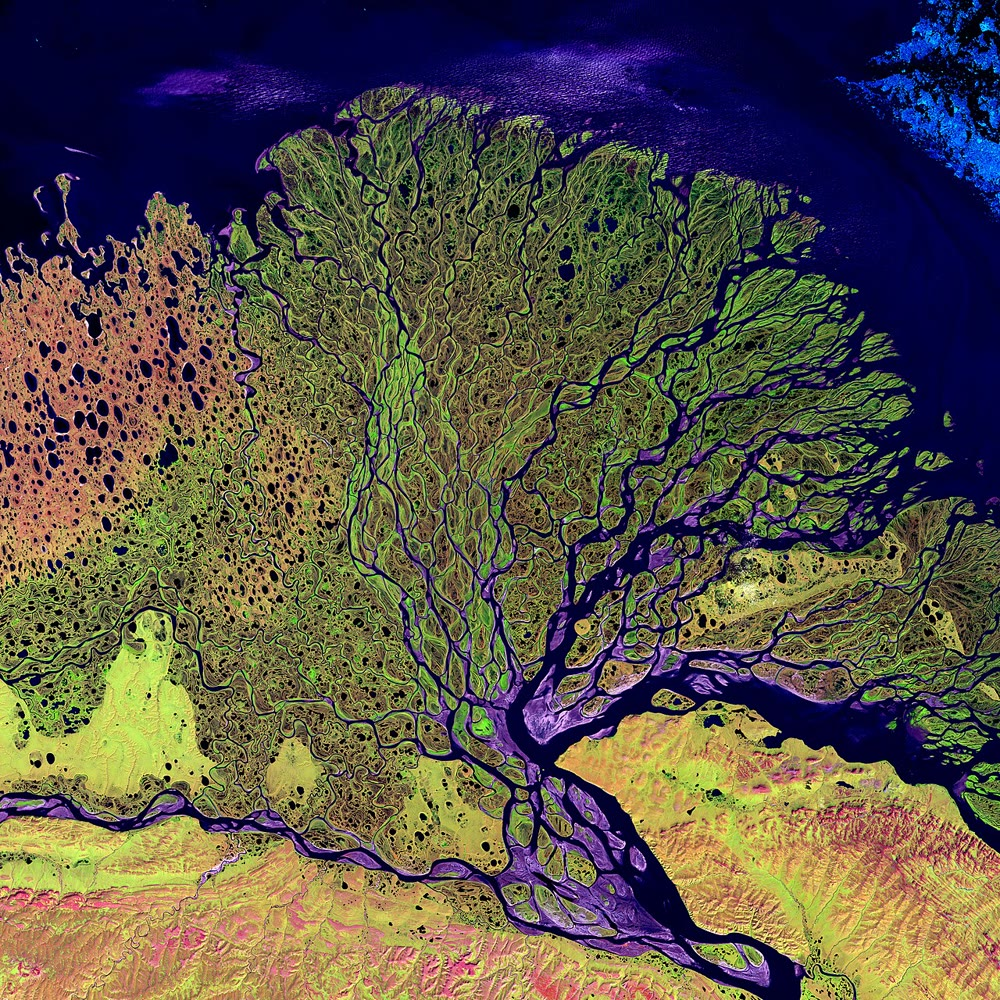
\includegraphics[width=\linewidth]{images/book1/g9-lena-delta.jpg}
\end{minipage}\hfill
\begin{minipage}[c]{0.46\linewidth}\raggedright
{\small El \omterm{def:g5:water-shapes-the-land:delta}{delta} del \omterm{def:g1:landscapes-around-us:water}{río} Lena, en Siberia, donde se encuentra con el \omterm{def:g2:water-on-earth:ocean}{océano}
Glacial Ártico: una imagen Landsat en falso color del 27~de febrero de
2000, obtenida con infrarrojo de onda corta, infrarrojo y luz roja. Los
numerosos brazos del \omterm{def:g1:landscapes-around-us:water}{río} aparecen en azul. USGS EROS Data Center, vía NASA
Visible Earth (dominio público, vía Wikimedia Commons).}
\end{minipage}
% ledger: commons:lena-landsat
\label{fig:g9:maps-of-the-earth:lena}
\end{omfigure}

\section{El posicionamiento por satélite}

Un teléfono o un coche pueden saber dónde están con un margen de unos
pocos metros, casi en cualquier lugar de la Tierra. No ven los satélites:
los escuchan.

\begin{definition}[Posicionamiento por satélite]\label{def:g9:maps-of-the-earth:positioning}
El \emph{posicionamiento por satélite}\index{posicionamiento por satelite@posicionamiento por satélite}
consiste en determinar una posición en la Tierra a partir de las
distancias a varios satélites cuyas posiciones se conocen. Un receptor
calcula cada distancia a partir del tiempo que tarda en llegarle una señal
del satélite.
\end{definition}

El sistema estadounidense, el GPS, mantiene al menos 24 satélites en
funcionamiento a una \omterm{def:g4:world-physical-map:altitude}{altitud} de unos \qty{20200}{km}. Cada uno da dos
vueltas a la Tierra al día, en seis órbitas repartidas alrededor del
planeta, de modo que desde casi cualquier punto de la Tierra hay al menos
cuatro satélites a la vista. Una señal procedente de \qty{20200}{km}, que
viaja a la velocidad de la luz, llega al cabo de $20\,200 \div
300\,000 \approx 0.067$~s: el receptor mide este tiempo y lo convierte en
una distancia.
% ledger: gps:constellation, const:c (travel time computed in figdata/grade-9/trilateration.py)

¿Cómo dan una posición las distancias? Imaginemos la idea en un mapa
plano. Si el receptor está a \qty{5}{km} de la baliza~A, se encuentra en
algún punto de un círculo de \qty{5}{km} de radio alrededor de A. Si está
además a \qty{10}{km} de B, se encuentra en los dos círculos: en uno de los
dos puntos donde se cortan. Una tercera distancia, \qty{5}{km} a C, elige
el bueno. En el espacio, los círculos se convierten en esferas, y hace
falta un satélite más por la misma razón.

\begin{omfigure}
\begin{minipage}[c]{0.5\linewidth}\centering
\begin{tikzpicture}
\begin{axis}[x=0.42cm, y=0.42cm, xmin=-1, xmax=13, ymin=-1.5, ymax=13,
  ticks=none, axis line style={black!40}]
  \addplot[omSea!70!black, line width=0.6pt] table {figdata/out/grade-9-trilateration-circles.dat};
  \addplot[only marks, mark=triangle*, mark size=2.6pt, point meta=explicit symbolic, nodes near coords,
    nodes near coords style={font=\footnotesize\bfseries, anchor=south west, inner sep=1pt}]
    table[meta=label] {figdata/out/grade-9-trilateration-beacons.dat};
  % labels first (on a white patch), then the points on top of them
  \addplot[only marks, mark=none, point meta=explicit symbolic, nodes near coords,
    nodes near coords style={font=\footnotesize\bfseries, anchor=north east, xshift=-1pt, yshift=-1pt, inner sep=1pt, fill=white, text=red!75!black}, skip coords between index={1}{2}]
    table[meta=label] {figdata/out/grade-9-trilateration-points.dat};
  \addplot[only marks, mark=none, point meta=explicit symbolic, nodes near coords,
    nodes near coords style={font=\footnotesize, anchor=south west, xshift=1pt, yshift=1pt, inner sep=1pt, fill=white}, skip coords between index={0}{1}]
    table[meta=label] {figdata/out/grade-9-trilateration-points.dat};
  \addplot[only marks, mark=*, mark size=2pt, red!75!black, skip coords between index={1}{2}] table {figdata/out/grade-9-trilateration-points.dat};
  \addplot[only marks, mark=o, mark size=2pt, fill=white, skip coords between index={0}{1}] table {figdata/out/grade-9-trilateration-points.dat};
\end{axis}
\end{tikzpicture}
\end{minipage}\hfill
\begin{minipage}[c]{0.46\linewidth}\raggedright
{\small El posicionamiento en un mapa plano (un esquema; no se dibuja la
cuadrícula en kilómetros). El receptor R está a \qty{5}{km} de A, a
\qty{10}{km} de B y a \qty{5}{km} de C. Los círculos alrededor de A y de B
se cortan en R y en un punto falso F; solo R está también en el círculo
alrededor de C.}
\end{minipage}
% ledger: (invented region: exercise data, figdata/grade-9/trilateration.py)
\label{fig:g9:maps-of-the-earth:trilateration}
\end{omfigure}

\begin{omfigure}
\begin{minipage}[t]{0.48\linewidth}\centering
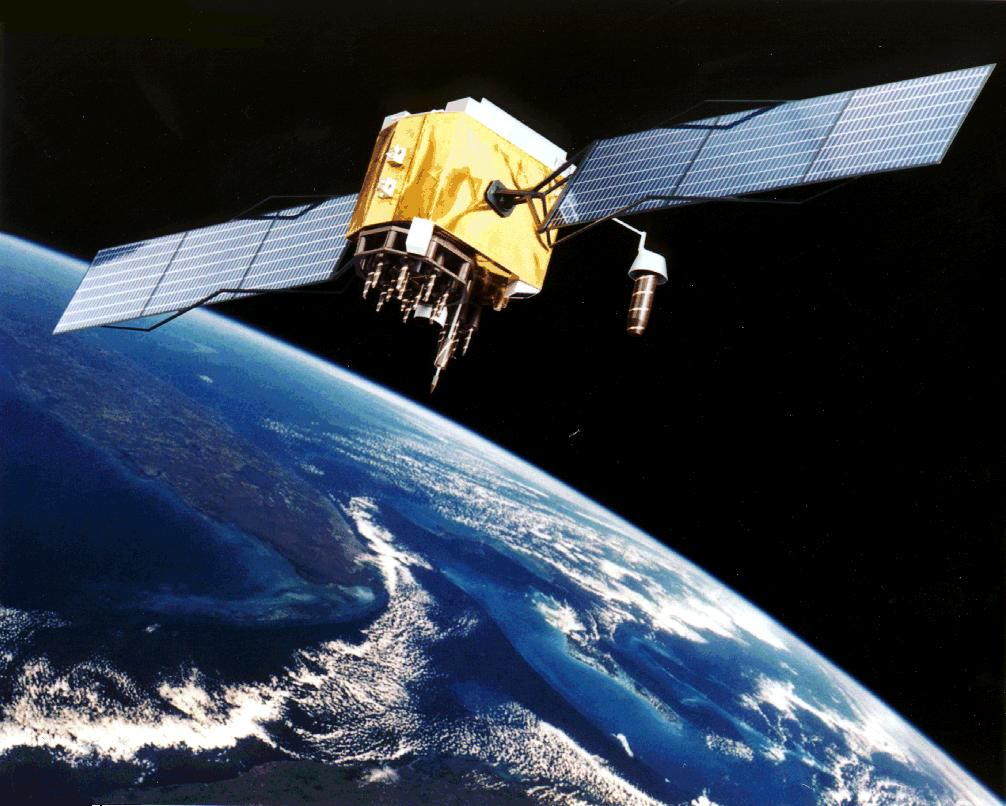
\includegraphics[width=\linewidth]{images/book1/g9-gps-satellite.jpg}

{\small Un satélite GPS en órbita, tal como lo imaginó un artista. NASA
(dominio público, vía Wikimedia Commons).}
\end{minipage}\hfill
\begin{minipage}[t]{0.48\linewidth}\centering
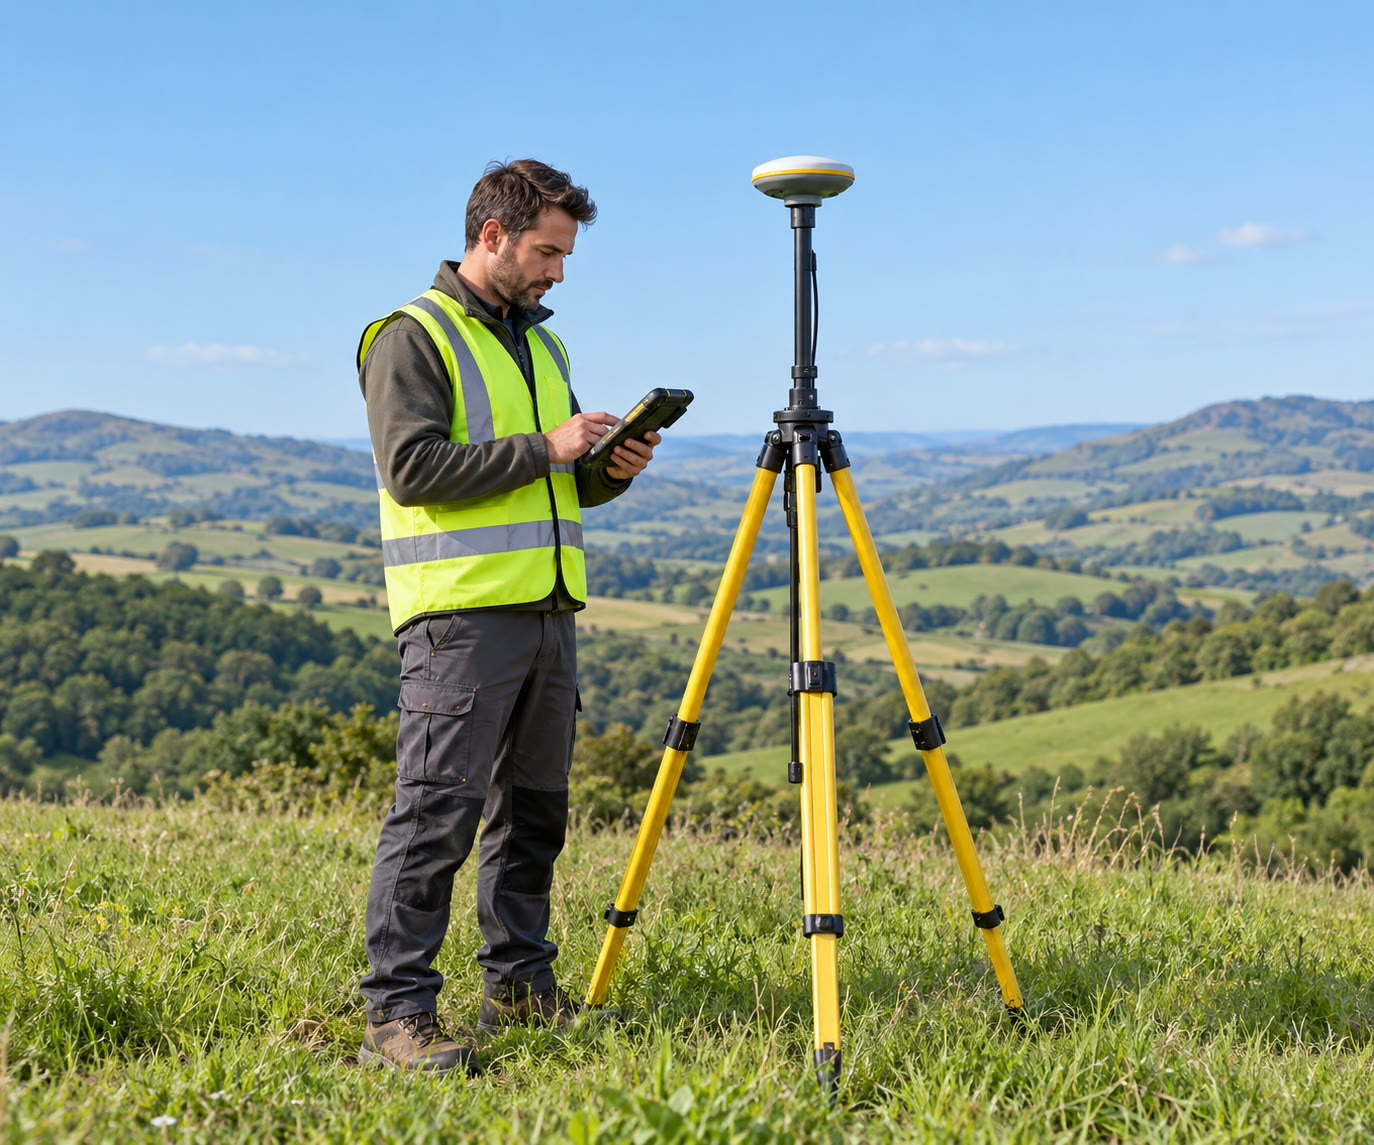
\includegraphics[width=\linewidth]{images/book1/ai/g9-surveyor.jpg}

{\small Un topógrafo fija la posición de un punto con un receptor de
satélite montado en un trípode (una ilustración).}
\end{minipage}
% ledger: commons:gps-iif
\label{fig:g9:maps-of-the-earth:gps}
\end{omfigure}

\section{Ejercicios}

\begin{exercise}[$\star$]\label{exo:g9:maps-of-the-earth:1}
Da la palabra que corresponde a cada descripción. (a) Una regla que envía
cada punto del \omterm{def:g3:continents-and-oceans:globe}{globo} a un punto de un mapa plano. (b) Una línea que une
puntos situados a la misma \omterm{def:g4:world-physical-map:altitude}{altitud}. (c) Una razón como $1 : 50\,000$.
(d) La diferencia de \omterm{def:g4:world-physical-map:altitude}{altitud} entre dos \omterm{def:g9:maps-of-the-earth:contour}{curvas de nivel} vecinas.
(e) Observar la Tierra a distancia, por ejemplo desde un satélite.
\end{exercise}

\begin{exercise}[$\star$]\label{exo:g9:maps-of-the-earth:2}
Convierte cada distancia del \omterm{def:g2:drawing-to-map:map}{mapa} en una distancia sobre el terreno, en
metros o kilómetros. (a) \qty{4}{cm} en un \omterm{def:g2:drawing-to-map:map}{mapa} a $1 : 25\,000$.
(b) \qty{3}{cm} en un \omterm{def:g2:drawing-to-map:map}{mapa} a
$1 : 50\,000$. (c) \qty{2.5}{cm} en un \omterm{def:g2:drawing-to-map:map}{mapa} a $1 : 1\,000\,000$. (d) En un
\omterm{def:g2:drawing-to-map:map}{mapa} a
$1 : 25\,000$, ¿cuántos centímetros representan \qty{1}{km}?
\end{exercise}

\begin{exercise}[$\star$]\label{exo:g9:maps-of-the-earth:3}
¿Verdadero o falso? Corrige las frases falsas. (a) Un \omterm{def:g3:continents-and-oceans:world-map}{mapamundi} puede
mostrar toda la Tierra sin deformar nada. (b) En un \omterm{def:g2:drawing-to-map:map}{mapa} de Mercator,
Groenlandia parece más grande de lo que es. (c) En un \omterm{def:g2:drawing-to-map:map}{mapa} equivalente,
las formas se conservan en todas partes. (d) Una \omterm{def:g9:maps-of-the-earth:numerical-scale}{escala gráfica} sigue
siendo correcta cuando se amplía un \omterm{def:g2:drawing-to-map:map}{mapa} en una fotocopiadora.
\end{exercise}

\begin{exercise}[$\star$]\label{exo:g9:maps-of-the-earth:4}
En un \omterm{def:g9:maps-of-the-earth:topographic-map}{mapa topográfico}, (a) ¿qué significa que las \omterm{def:g9:maps-of-the-earth:contour}{curvas de nivel} estén
muy juntas? (b) ¿Y que estén muy separadas? (c) ¿Qué muestran unas \omterm{def:g9:maps-of-the-earth:contour}{curvas
de nivel} cerradas que suben hacia el interior? (d) ¿Por qué no pueden
cortarse nunca dos \omterm{def:g9:maps-of-the-earth:contour}{curvas de nivel}?
\end{exercise}

\begin{exercise}[$\star\star$]\label{exo:g9:maps-of-the-earth:5}
% ledger: data:ne-land (factor 1/cos^2, figdata/grade-9/projections.py)
En un \omterm{def:g2:drawing-to-map:map}{mapa} de Mercator, las superficies situadas a la \omterm{def:g6:latitude-longitude:latitude}{latitud} de \ang{60}
se agrandan 4 veces, y a la \omterm{def:g6:latitude-longitude:latitude}{latitud} de \ang{30} unas 1.33 veces, en
comparación con el \omterm{def:g3:continents-and-oceans:equator}{ecuador}. (a) Se dibuja en el \omterm{def:g2:drawing-to-map:map}{mapa} un \omterm{def:g1:landscapes-around-us:water}{lago} de
\qty{1000}{km^2} situado a \ang{60}\,N. ¿Qué superficie real tiene un \omterm{def:g1:landscapes-around-us:water}{lago}
del \omterm{def:g3:continents-and-oceans:equator}{ecuador} dibujado con el mismo tamaño? (b) Dos islas de la misma
superficie real están a \ang{30} y a \ang{60}. ¿Cuántas veces más grande
parece la segunda que la primera? (c) ¿Por qué el \omterm{def:g2:drawing-to-map:map}{mapa} de Mercator nunca
puede mostrar los \omterm{def:g3:continents-and-oceans:poles}{polos}?
\end{exercise}

\begin{exercise}[$\star\star$]\label{exo:g9:maps-of-the-earth:6}
% ledger: (invented region: the Varden Hills map of the chapter)
Usa el \omterm{def:g9:maps-of-the-earth:topographic-map}{mapa topográfico} de las Colinas de Varden de este capítulo. (a) ¿Cuál
es la \omterm{def:g9:maps-of-the-earth:contour}{equidistancia}? (b) ¿Cuál es la \omterm{def:g4:world-physical-map:altitude}{altitud} de la cima marcada con su
cota, y la de la curva maestra que la rodea? (c) El \omterm{def:g1:landscapes-around-us:water}{río} fluye hacia el
este. ¿Está más alto el fondo del \omterm{def:g1:landscapes-around-us:landform}{valle} en el oeste o en el este del \omterm{def:g2:drawing-to-map:map}{mapa}?
(d) A lo largo de C--D, al norte del \omterm{def:g1:landscapes-around-us:water}{río}, ¿entre qué \omterm{def:g9:maps-of-the-earth:contour}{curvas de nivel} están
las líneas más juntas? ¿Qué te dice eso sobre la pendiente en ese lugar?
\end{exercise}

\begin{exercise}[$\star\star$]\label{exo:g9:maps-of-the-earth:7}
% ledger: (invented region: profile C--D, figdata/grade-9/varden_topo.py)
Usa el perfil C--D de este capítulo. (a) ¿A qué \omterm{def:g4:world-physical-map:altitude}{altitud} aproximada están C
y D? (b) ¿Cuál es la \omterm{def:g4:world-physical-map:altitude}{altitud} más baja a lo largo del perfil, y a qué
distancia de C está? (c) ¿Qué longitud tiene el fondo llano del \omterm{def:g1:landscapes-around-us:landform}{valle} a lo
largo de C--D? (d) El perfil está dibujado con su escala vertical exagerada
tres veces. ¿Por qué lo hacen a menudo los cartógrafos?
\end{exercise}

\begin{exercise}[$\star\star$]\label{exo:g9:maps-of-the-earth:8}
En un \omterm{def:g2:drawing-to-map:map}{mapa} a $1 : 25\,000$, un camino cruza la curva de \qty{200}{m} y
después la de \qty{300}{m}, \qty{2}{cm} más allá. (a) ¿Cuál es la
distancia horizontal entre los dos puntos sobre el terreno? (b) ¿Cuánto
sube el camino? (c) ¿Cuál es la pendiente, en tanto por ciento? (d) Más
adelante, dos curvas separadas \qty{100}{m} en \omterm{def:g4:world-physical-map:altitude}{altitud} están a
\qty{4}{cm} una de otra en el \omterm{def:g2:drawing-to-map:map}{mapa}. ¿Es allí el camino más empinado o más
suave? ¿En qué proporción?
\end{exercise}

\begin{exercise}[$\star\star$]\label{exo:g9:maps-of-the-earth:9}
% ledger: usgs:landsat1
El Landsat~1 daba 14 vueltas a la Tierra al día y pasaba sobre el mismo
lugar cada 18 días. (a) ¿Cuántas órbitas completaba entre dos pasos sobre
el mismo lugar? (b) Cada órbita duraba 103 minutos. ¿Cuánto duran, en
horas, 14 órbitas? (c) Construido para funcionar un año, se apagó el
6~de enero de 1978, cinco años y medio después de su lanzamiento. ¿Cuántas
veces su vida prevista funcionó? (d) Da un cambio de la superficie
terrestre que pueden mostrar las imágenes de un mismo lugar tomadas con
años de diferencia.
\end{exercise}

\begin{exercise}[$\star\star$]\label{exo:g9:maps-of-the-earth:10}
% ledger: gps:constellation, const:c
Un satélite GPS está a unos \qty{20200}{km}; su señal viaja a unos
\qty{300000}{km} por segundo. (a) ¿Cuánto tarda la señal en llegar?
Escribe la respuesta en notación científica. (b) Si el reloj de un
receptor se equivocara en $1 \times 10^{-3}$~s, ¿qué error causaría en la
distancia? (c) ¿Qué te dice esto sobre los relojes que se usan en el
\omterm{def:g9:maps-of-the-earth:positioning}{posicionamiento por satélite}?
\end{exercise}

\begin{exercise}[$\star\star\star$]\label{exo:g9:maps-of-the-earth:11}
En un mapa plano con una cuadrícula en kilómetros, la baliza A está en
$(0, 0)$ y la baliza B en $(10, 0)$. Un receptor está a \qty{6}{km} de A y
a \qty{8}{km} de B. (a) Demuestra que el punto $(3.6, 4.8)$ está a
\qty{6}{km} de A y a \qty{8}{km} de B. (b) Da otro punto situado a las
mismas distancias de A y de B. (c) Una tercera baliza C está en $(0, 10)$,
y el receptor está a unos \qty{6.3}{km} de ella. ¿Cuál de los dos puntos
es el receptor? (d) ¿Por qué el \omterm{def:g9:maps-of-the-earth:positioning}{posicionamiento por satélite} necesita
varios satélites?
\end{exercise}

\begin{exercise}[$\star\star\star$]\label{exo:g9:maps-of-the-earth:12}
% ledger: data:ne-land (areas, figdata/grade-9/projections.py)
El \omterm{def:g3:continents-and-oceans:continent}{continente} africano cubre unos 29~millones de~\unit{km^2}, y
Groenlandia unos 2.1~millones de~\unit{km^2}. (a) ¿Cuántas veces mayor es
África? (b) En un \omterm{def:g2:drawing-to-map:map}{mapa} de Mercator, las superficies cercanas al centro de
Groenlandia, a unos \ang{72}\,N, se agrandan unas 10.5 veces. Estima la
superficie que parece tener Groenlandia. (c) África se extiende a ambos
lados del \omterm{def:g3:continents-and-oceans:equator}{ecuador}, donde las superficies se agrandan poco. Compara tu
respuesta a (b) con la superficie de África, y explica el \omterm{def:g2:drawing-to-map:map}{mapa} mural del
principio del capítulo. (d) ¿Qué proyección elegirías para mostrar con
justicia el tamaño de los \omterm{def:g3:continents-and-oceans:continent}{continentes}?
\end{exercise}

\section{Problema: un sendero a través de las Colinas de Varden}

\begin{problem}[{Problema de fin de semana --- unos planificadores han
trazado un sendero a través de las Colinas de Varden en el mapa
topográfico; la respuesta final es la longitud del sendero en kilómetros y
su desnivel total de subida en metros}]
\label{pb:g9:maps-of-the-earth:1}
% ledger: (invented region: the Varden Hills, figdata/grade-9/varden_topo.py, part problem: leg lengths 3.6 / 2.5 / 2.35 cm, spot heights 296 / 143 / 335 / 544 m, 4.2 km, 401 m)
El sendero sale de una granja S, baja hasta un puente B sobre el \omterm{def:g1:landscapes-around-us:water}{río}, sube
después hasta un refugio W y sigue hasta la cima T. Cada tramo es recto y
solo baja o solo sube. El \omterm{def:g2:drawing-to-map:map}{mapa} está a $1 : 50\,000$; las \omterm{def:g4:world-physical-map:altitude}{altitudes} de S,
B, W y T están escritas a su lado.

\begin{omfigure}
\begin{tikzpicture}
\begin{axis}[x=1.6cm, y=1.6cm, xmin=2, xmax=8, ymin=1.8, ymax=6.2, ticks=none,
  axis line style={black!60}, clip mode=individual]
  \addplot[contour] table {figdata/out/shared-region-contours.dat};
  \addplot[index contour] table {figdata/out/shared-region-index-contours.dat};
  \addplot[river] table {figdata/out/shared-region-river.dat};
  \addplot[only marks, mark=none, point meta=explicit symbolic, nodes near coords,
    nodes near coords align={center}, nodes near coords style={font=\tiny, fill=white, inner sep=0.6pt, text=omContour}]
    table[meta=label] {figdata/out/grade-9-varden_topo-labels.dat};
  \addplot[red!75!black, line width=1pt, dashed] table[x=x_km, y=y_km] {figdata/out/grade-9-varden_topo-path.dat};
  \addplot[only marks, mark=*, mark size=1.6pt, red!75!black, point meta=explicit symbolic, nodes near coords,
    nodes near coords align={right}, nodes near coords style={font=\scriptsize\bfseries, text=black, fill=white, fill opacity=0.8, text opacity=1, inner sep=1pt}]
    table[meta=label] {figdata/out/grade-9-varden_topo-points.dat};
  \coordinate (na) at (axis cs:8.35,5.4);
\end{axis}
\pic at (na) {northarrow};
\end{tikzpicture}

{\small El sendero S--B--W--T en el \omterm{def:g9:maps-of-the-earth:topographic-map}{mapa topográfico} de las Colinas de
Varden (aquí reducido; en el \omterm{def:g2:drawing-to-map:map}{mapa} original a $1 : 50\,000$, los tramos
miden 3.6, 2.5 y \qty{2.35}{cm}).}
\label{fig:g9:maps-of-the-earth:path}
\end{omfigure}

\noindent\textbf{Parte I --- La ruta en el mapa.}\par\nopagebreak
\begin{enumerate}[beginpenalty=10000]
  \item A $1 : 50\,000$, ¿cuántos metros sobre el terreno representa
        \qty{1}{cm} del \omterm{def:g2:drawing-to-map:map}{mapa}?
  \item En el \omterm{def:g2:drawing-to-map:map}{mapa} original, el tramo S--B mide \qty{3.6}{cm}. ¿Qué
        longitud tiene sobre el terreno, en kilómetros?
  \item Los tramos B--W y W--T miden \qty{2.5}{cm} y \qty{2.35}{cm}. ¿Qué
        longitud tienen sobre el terreno?
  \item ¿En qué dirección general va el sendero de B a T?
\end{enumerate}

\noindent\textbf{Parte II --- La subida.}\par\nopagebreak
\begin{enumerate}[resume, beginpenalty=10000]
  \item ¿Cuál es la \omterm{def:g9:maps-of-the-earth:contour}{equidistancia} del \omterm{def:g2:drawing-to-map:map}{mapa}?
  \item ¿Qué tramo baja? ¿Cuántos metros?
  \item ¿Cuántos metros sube el sendero en B--W, y en W--T?
  \item ¿Cuál es la pendiente media del tramo W--T, en tanto por ciento?
  \item ¿Por qué los planificadores no trazaron el sendero en línea recta
        de S a T?
\end{enumerate}

\noindent\textbf{Parte III --- La caminata.}\par\nopagebreak
\begin{enumerate}[resume, beginpenalty=10000]
  \item Supón que un excursionista recorre \qty{4}{km} por hora en llano y
        necesita un minuto más por cada \qty{10}{m} de subida. ¿Cuánto
        dura toda la caminata?
  \item Otra excursionista recorre el sendero en sentido contrario, de T a
        S. ¿Cuántos metros sube?
  \item ¿Cuál es la longitud total del sendero, en kilómetros, y su
        desnivel total de subida, en metros?
\end{enumerate}
\end{problem}
